% Solvers in ug4

\section {Coupling equations in ug4}

\begin {frame} [t]
\frametitle {Systems of PDEs: coupling of equations}
\vspace{-4ex}
$$
	\left \{
	 \begin{array} {c}
	  \mathcal{A}^{(1)} (u^{(1)}\uncover<3->{, f^{(1)} (u^{(2)})}) = 0 \\
	  \uncover<2->{\mathcal{A}^{(2)} (u^{(2)}\uncover<3->{, f^{(2)} (u^{(1)})}) = 0}
	 \end{array}
	\right .
	\qquad
	\uncover<6->
	{
	\equiv
	 \mathcal{A} (u) = 0, \quad u := (u^{(1)}, u^{(2)})^{\top}
	}
$$

\vspace{-2ex}
\begin {itemize}
\item<4-> {\color{blue} Loose coupling}: The eq's are solved one-by-one, without iterating.
	\begin {itemize}
		\item Advantages: Requires only scalar discretizations
		\item Disadvantage: Stability restrictions on the time step
	\end {itemize}
\item<5-> {\color{blue} Iterative (sequential) coupling}: The eq's are
	solved one by one with fixing the unknowns in the ``inactive'' eq's. This
	process is iterated ``until converged''.
	\begin {itemize}
		\item Advantages: Requires only scalar discretizations
		\item Disadvantage: Time-step dependent convergence
	\end {itemize}
\item<6-> {\color{blue} Full (monolithic) coupling}: The system is treated as a whole and discretized to
	a single big system of algebraic equations.
	\begin {itemize}
		\item Advantages: Stability (e.g. via implicit time disc. etc.)
		\item Disadvantage: Big non-linear discretized systems 
	\end {itemize}
\end {itemize}
\end {frame}

\begin {frame} [t]
\frametitle {Coupling in ug4}
In ug4, main the monolitic coupling is used.
\centerline {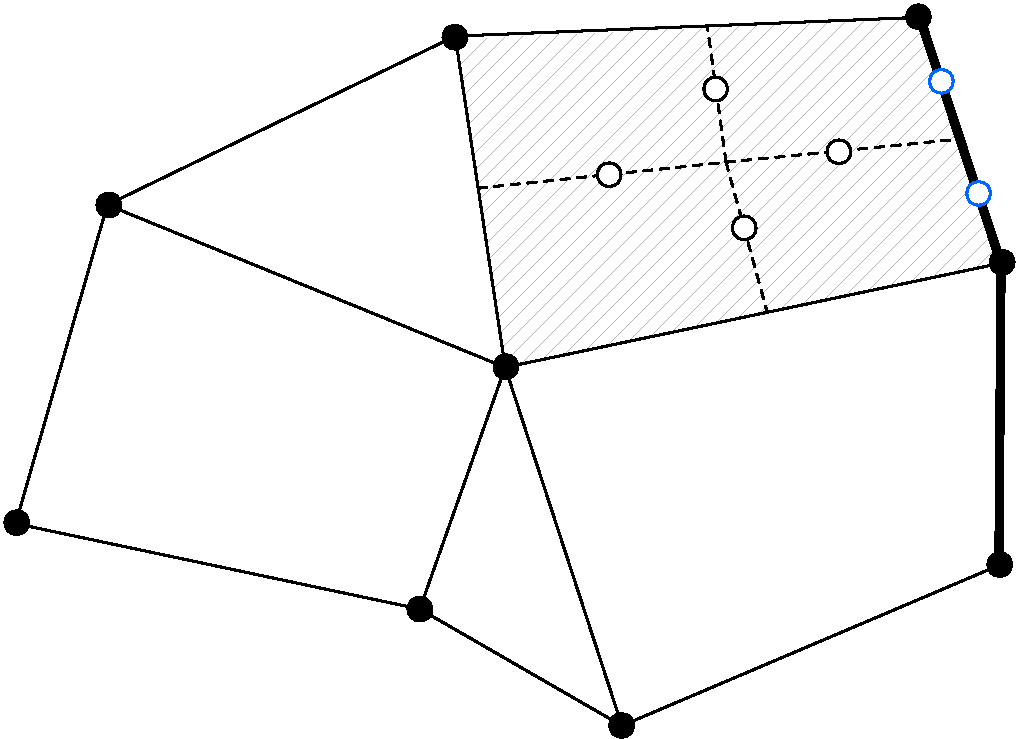
\includegraphics [width=0.6\textwidth] {DiscDetails-Local.pdf}}
The coupling happens on the level of DomainDiscretization. In every element, local
discretizations are used independently. The data $f^{(i)} (u^{(k)})$ are exchanged
in the integration points using objects of ``{\color{blue} UserData}'' class.
\end {frame}

\begin {frame} [t]
\frametitle {Full coupling in ug4}
\vspace{-2ex}
\begin {itemize}
\item Local (``element'') discretizations declare {\color{blue} export parameters}
	(e.g. velocity). These parameters may be the unknowns or functions of unknowns.
\pause
\item Local discretizations declare {\color{blue} import parameters}, i.e. values
	required in the coefficients of the equations.
\pause
\item All the local discretizations are added to the same global (``domain'') discretization.
	export parameters of some discretizations may be associated with (``plugged into'')
	import parameters of other discretizations.
\pause
\item Instead of the direct association, connection via the
	s.c. ``{\color{blue} linkers}'' (objects that transform values) can be used.
\pause
\item The global discretization assembles one big algebraic system. {\color{blue} Before}
	assembling local matrices and defects in every element, the export parameters are
	evaluated and transfered to the import parameters.
\end {itemize}
\end {frame}

\begin {frame} [t]
\frametitle {Computation of the defect}
\only<1>{\flushleft {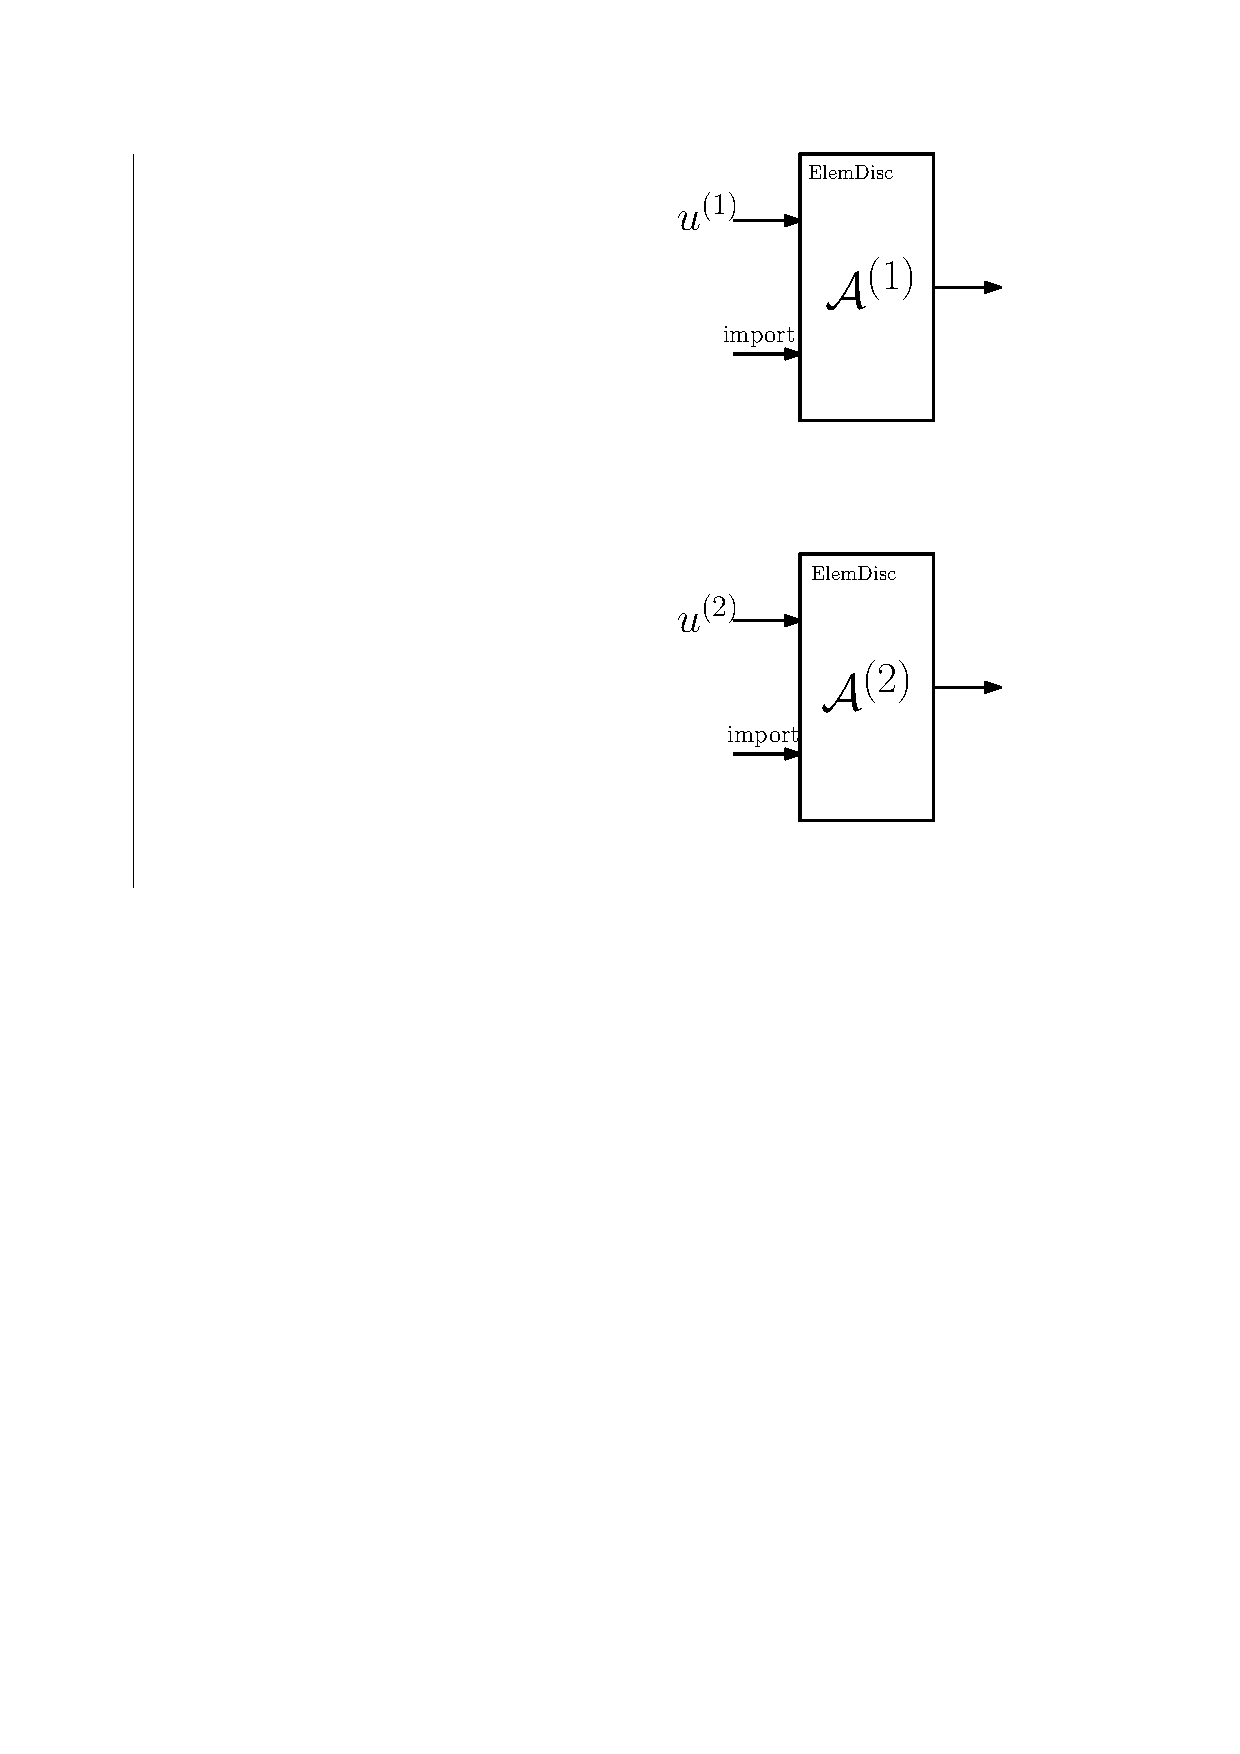
\includegraphics [width=0.7\textwidth] {ug4-coupling-scheme.pdf}}}%
\only<2>{\flushleft {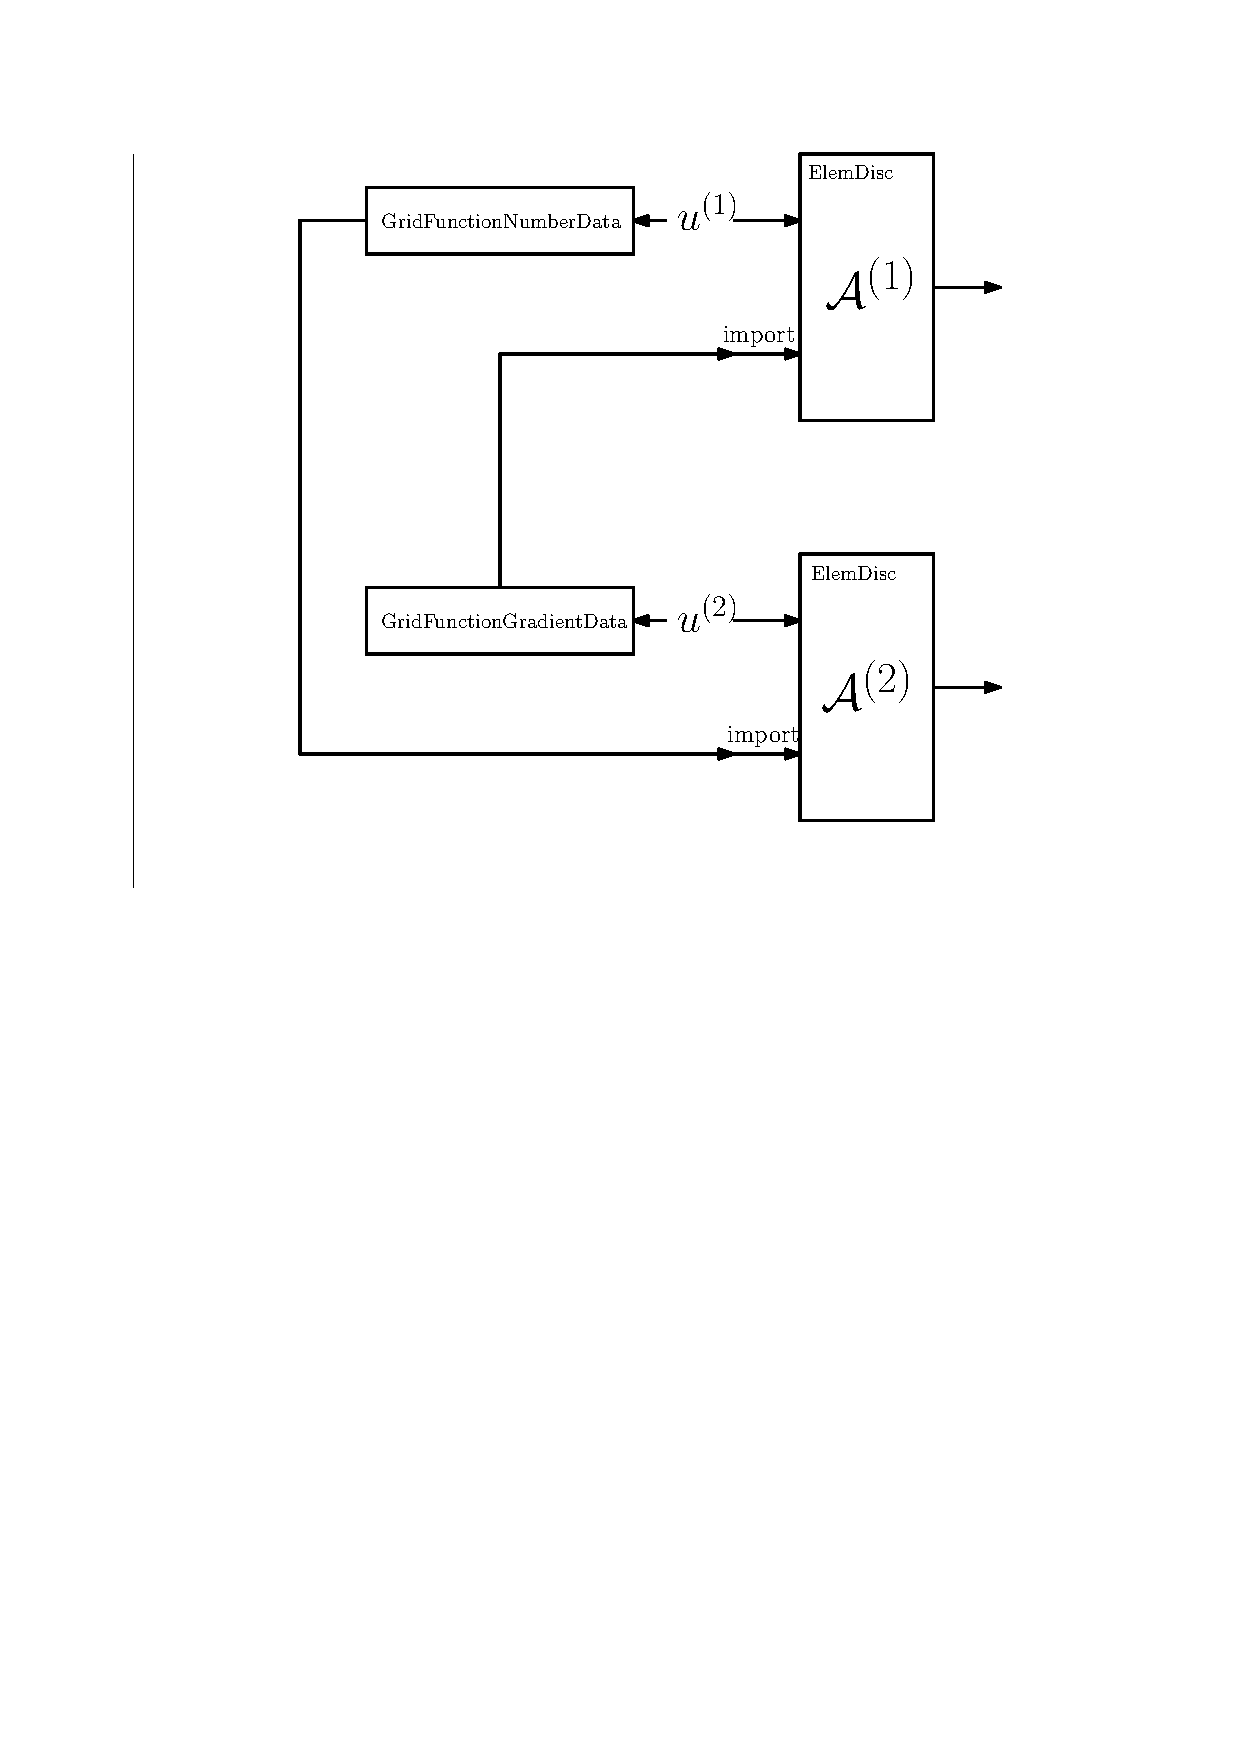
\includegraphics [width=0.7\textwidth] {ug4-coupling-scheme-simple.pdf}}}%
\only<3>{\flushleft {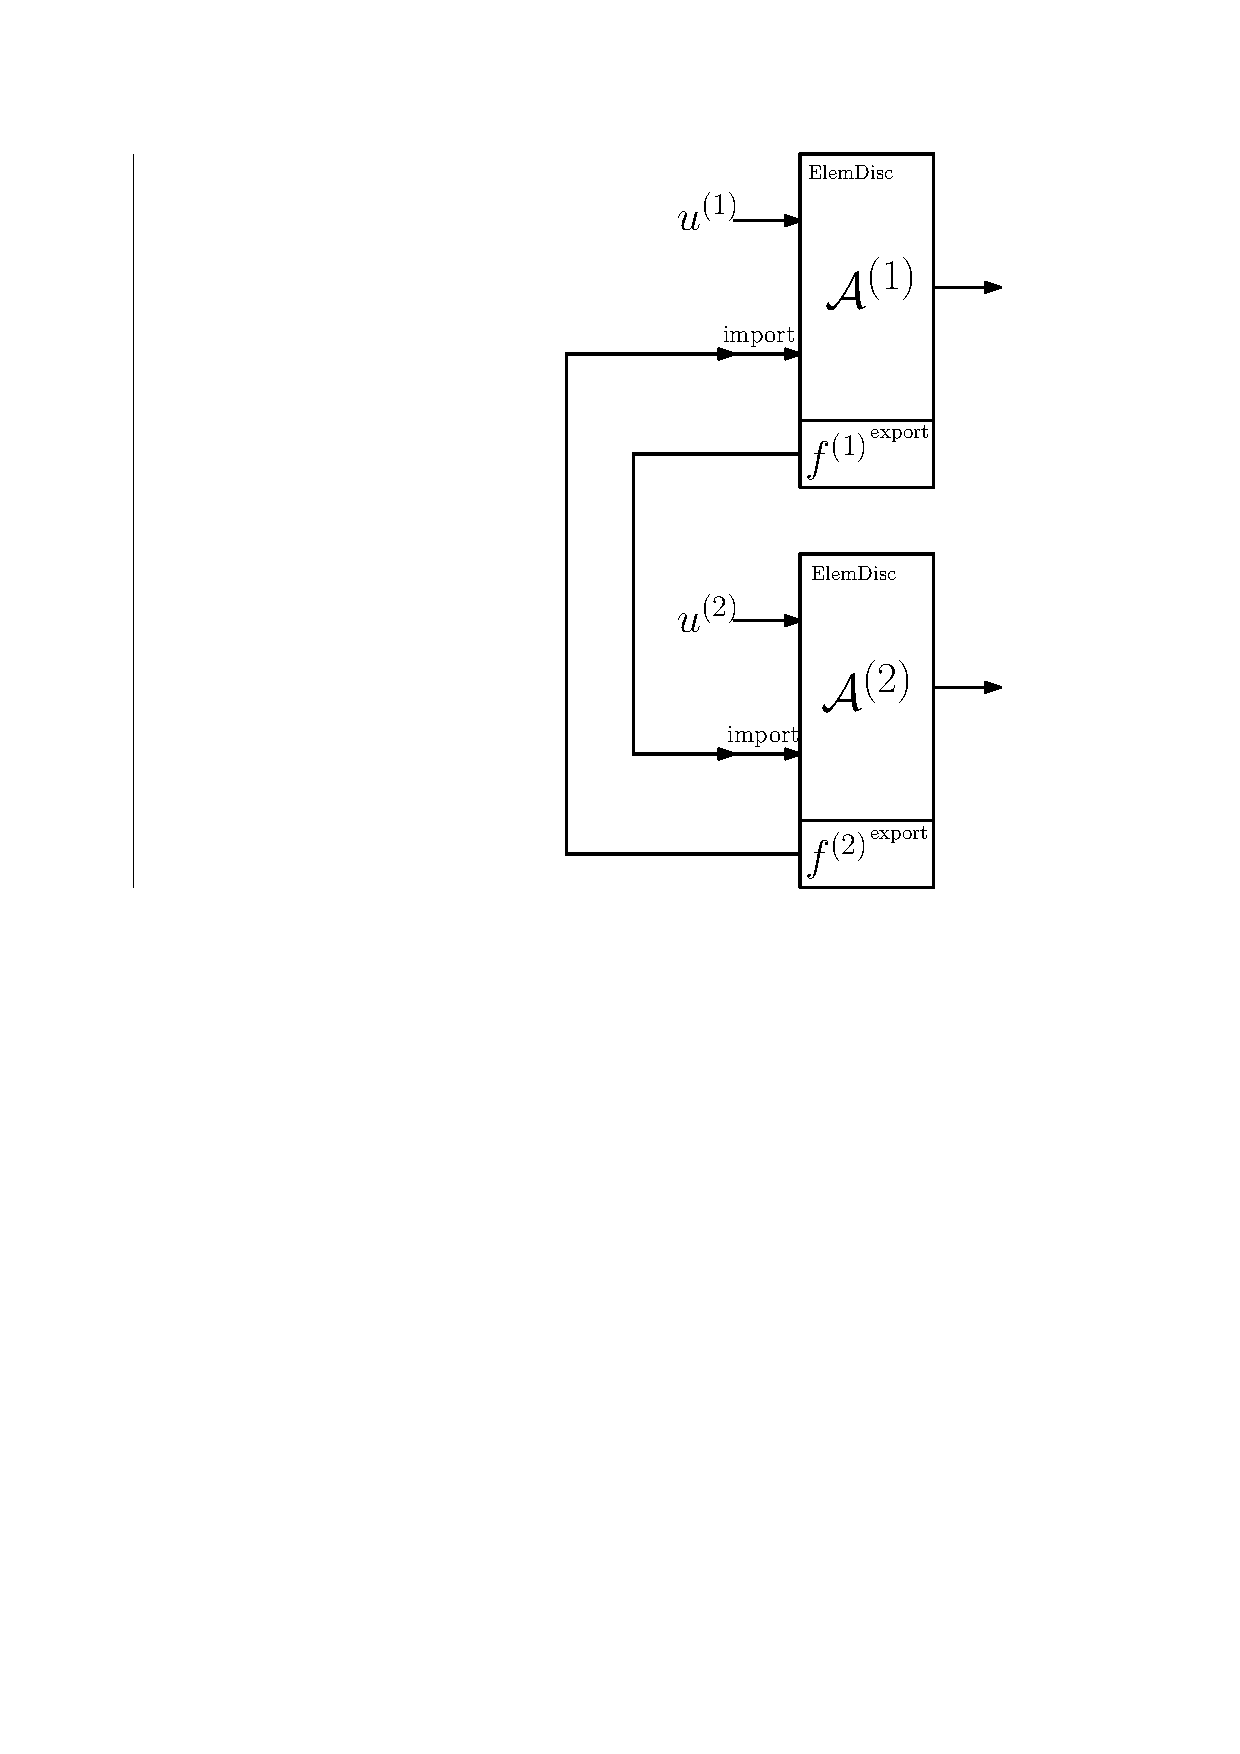
\includegraphics [width=0.7\textwidth] {ug4-coupling-scheme-export.pdf}}}%
\only<4>{\flushleft {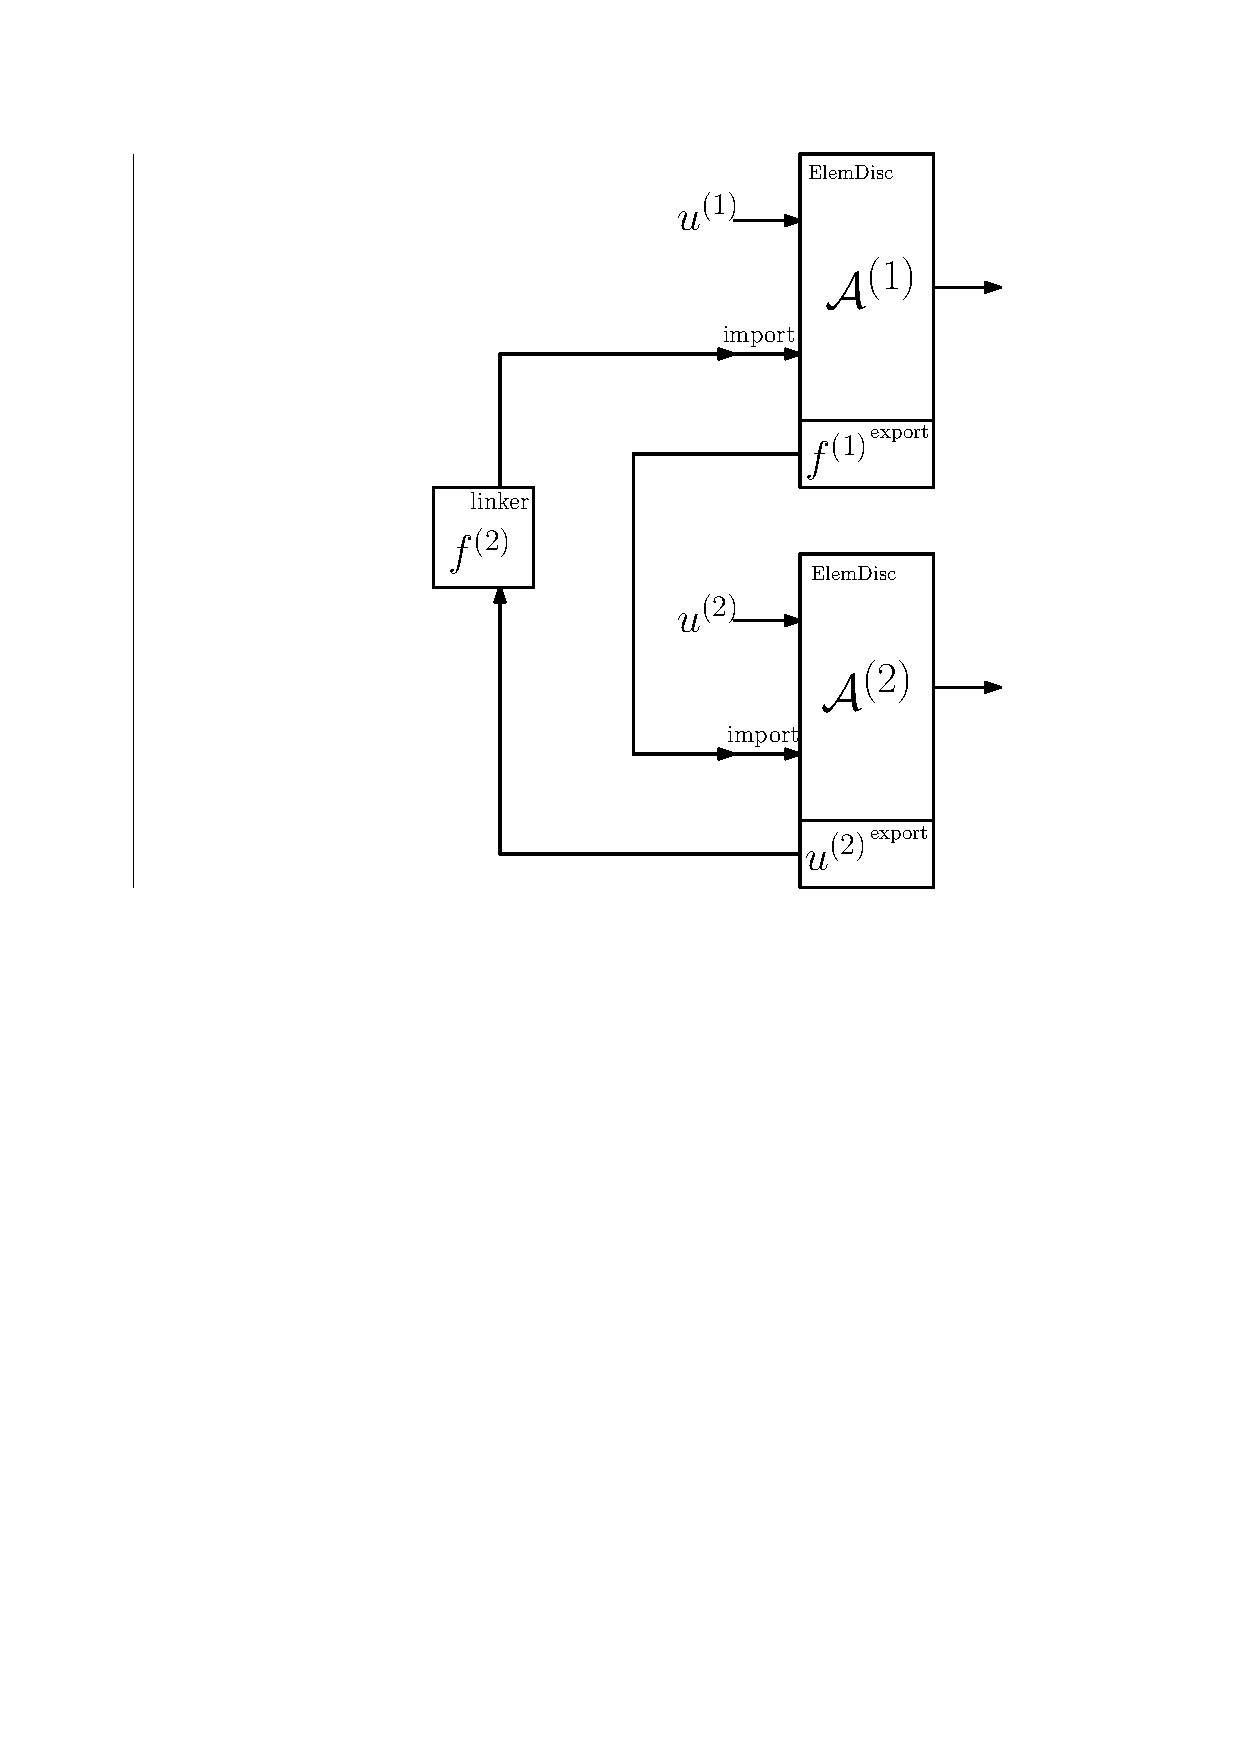
\includegraphics [width=0.7\textwidth] {ug4-coupling-scheme-linker.pdf}}}%
\end {frame}

\begin {frame} [t]
\frametitle {Data interfaces}
\begin {itemize}
	\item Data exchange is implemented using the {\color{blue} UserData} class.
	\item Discretizations require data at ``{\color{blue} local ip series}''. UserData
	 with registered local ip series is ``{\color{blue} CplUserData}''.
	\item From CplUserData, classes DataExport (for exports), StdDataLinker (for linkers) etc. derived.
	\item CplUserData that implement derivatives are called ``{\color{blue} DependentUserData}''.
	\pause
	\item Currently, UserData class does not provide grid-element-type specific computations.
	 DataExports implements its own engine for that.
\end {itemize}
\end {frame}

\begin {frame} [t]
\frametitle {Jacobians of coupled operators}
$$
 \mathbf{A} := \dfrac{\partial{\mathcal{A}}}{\partial u} =
 \left (
  \begin {array} {cc}
   {\color{blue} \tfrac{\partial \mathcal{A}^{(1)} (u^{(1)}, f^{(1)} (u^{(2)}))}{\partial u^{(1)}}}
    & {\color{red} \tfrac{\partial \mathcal{A}^{(1)} (u^{(1)}, f^{(1)} (u^{(2)}))}{\partial u^{(2)}}} \\[1ex]
   {\color{red} \tfrac{\partial \mathcal{A}^{(2)} (u^{(2)}, f^{(2)} (u^{(1)}))}{\partial u^{(1)}}}
    & {\color{blue} \tfrac{\partial \mathcal{A}^{(2)} (u^{(2)}, f^{(2)} (u^{(1)}))}{\partial u^{(2)}}}
  \end {array}
 \right )
$$

\vspace{2ex}
\only<2>%
{%
{\color{blue} Blue terms} are computed in ElemDisc's: They are ``usual''
Jacobians for the uncoupled equations in the case of the fixed parameters.}
\only<3->%
{%
{\color{red} Red terms} are computed via the functions of the imports
and the connected exports, linkers etc.:
$$
 \tfrac{\partial \mathcal{A}^{(1)} (u^{(1)}, f^{(1)} (u^{(2)}))}{\partial u^{(2)}}
  = \underbrace{\partial_2 \mathcal{A}^{(1)} (u^{(1)}, f^{(1)} (u^{(2)}))}_{(a)}
   \cdot \underbrace{\partial f^{(1)} (u^{(2)})}_{(b)}
$$
$(a)$ is evaluated by ``lin\_defect'' functions of the import parameter,

$(b)$ is computed by the DependentUserData object.
}

\only<4>%
{%
Position of the off-diagonal entries in the matrix is determined by ``{\color{blue} function pattern}''
of the DependentUserData class.
}
\only<5->%
{%
Computation of the off-diagonal terms can be suppressed
by the ``comp\_lin\_defect'' flag of the import.
}
\end {frame}

% End of File
